\documentclass[UTF8]{ctexart}
\usepackage[a4paper,margin=2.4cm]{geometry}
\usepackage{booktabs}
\usepackage{graphicx}
\usepackage{float}
\usepackage{hyperref}
\usepackage{caption}
\usepackage{amsmath}
\hypersetup{colorlinks=true,linkcolor=blue,urlcolor=blue}

\title{深度学习课程实验报告}
\author{}
\date{\today}

\begin{document}
\maketitle

\begin{abstract}
本报告围绕课程任务书中的三个实验展开：纯 NumPy 实现多层感知机、基于 PyTorch 的 MNIST 卷积神经网络、以及面向 MNIST 的 ResNet。除完成基础训练和预测流程外，本文进一步补充了较系统的超参数搜索与结构消融实验，包括学习率、优化器、激活函数、隐藏层宽度、卷积核大小、通道数、BatchNorm、Dropout、池化、ResNet 深度、残差连接和 stem 设计等因素。实验结果以 JSON、CSV、Markdown、图表和 LaTeX 表格形式保留，便于复现与汇报。
\end{abstract}

\section{实验目标与组织}
任务书要求按三个文件夹分别提交程序：\texttt{01\_numpy\_mlp}、\texttt{02\_mnist\_cnn}、\texttt{03\_resnet\_mnist}。本仓库保持这一结构，并将综合报告材料集中保存在 \texttt{latex\_report}，其中 \texttt{figures} 保存图像，\texttt{tables} 保存 LaTeX 表格。

\section{实验环境}
实验使用项目内隔离环境 \texttt{.conda-env}，Python 版本为 3.10，深度学习框架为 PyTorch 2.4.0 与 torchvision 0.19.0。CNN 与 ResNet 实验在 GPU 上训练，NumPy MLP 使用 CPU 完成全批量梯度更新。所有实验默认固定随机种子，并在输出文件中记录训练配置。

\section{实验一：NumPy MLP}
\subsection{方法}
第一题仅使用 NumPy 实现输入层、隐藏层、输出层、激活函数、Softmax 交叉熵损失和反向传播。基础版本使用 ReLU 和普通梯度下降；扩展实验比较 ReLU、Tanh、Sigmoid 三类激活函数，隐藏层宽度 16/32/64/128，学习率 0.1/0.05/0.01/0.005，以及 GD、Momentum、Adam 三类优化方式。排名靠前的配置进一步使用多个随机种子复验，降低偶然性。

\subsection{结果}
MLP 最优配置为 \texttt{relu} 激活、隐藏层 \texttt{16}、学习率 \texttt{0.01}、\texttt{adam} 优化器，测试准确率为 99.17\%。

\begin{table}[H]
\centering
\caption{MLP 超参数搜索靠前配置}
\begin{tabular}{llllll}
\toprule
激活 & 隐藏层 & 学习率 & 优化器 & 测试准确率 & 标准差 \\
\midrule
relu & 16 & 0.01 & adam & 99.17\% & 0.68\% \\
relu & 64 & 0.1 & momentum & 98.61\% & 0.79\% \\
relu & 16 & 0.05 & adam & 98.61\% & 0.39\% \\
relu & 64 & 0.1 & adam & 98.33\% & 0.68\% \\
relu & 64 & 0.05 & adam & 98.33\% & 0.68\% \\
\bottomrule
\end{tabular}

\end{table}

\begin{figure}[H]
\centering
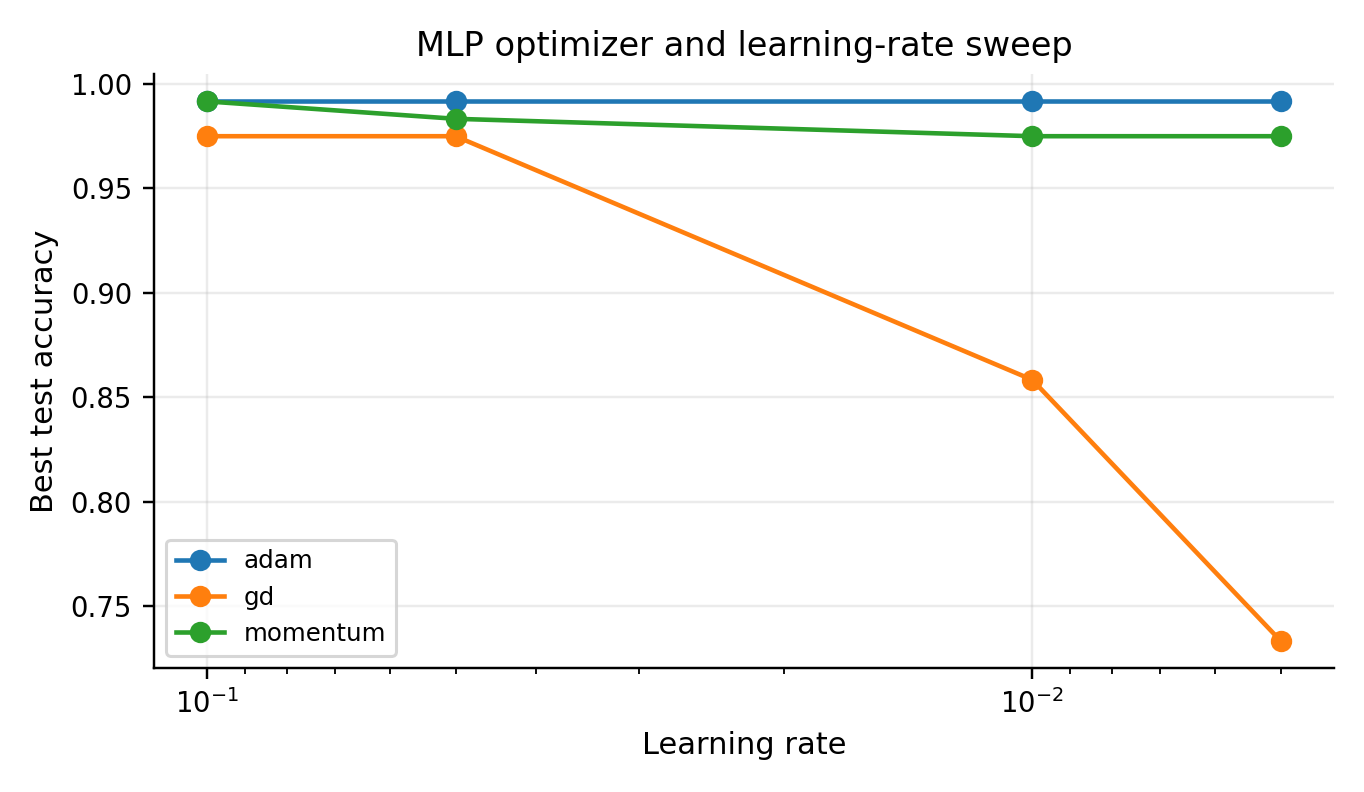
\includegraphics[width=0.72\linewidth]{figures/mlp_optimizer_lr.png}
\caption{MLP 不同优化器与学习率下的最佳测试准确率}
\end{figure}

\begin{figure}[H]
\centering
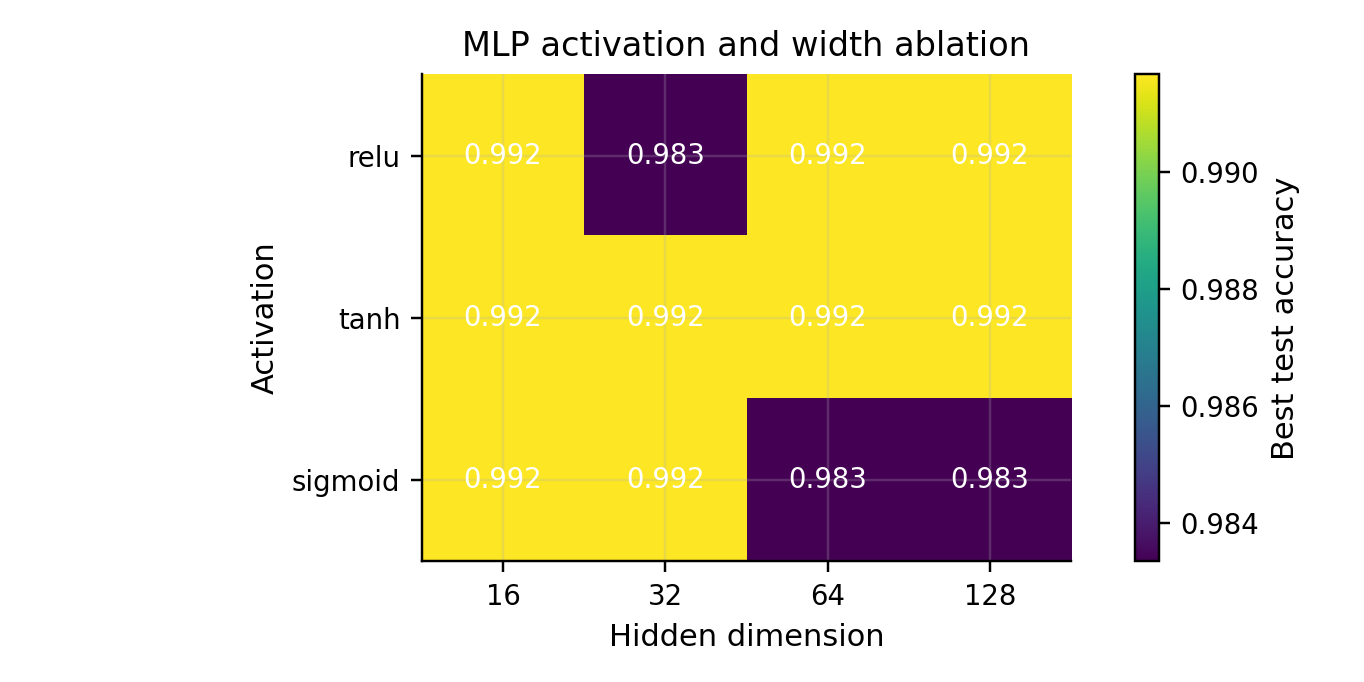
\includegraphics[width=0.72\linewidth]{figures/mlp_activation_hidden.png}
\caption{MLP 激活函数和隐藏层宽度消融}
\end{figure}

\begin{figure}[H]
\centering
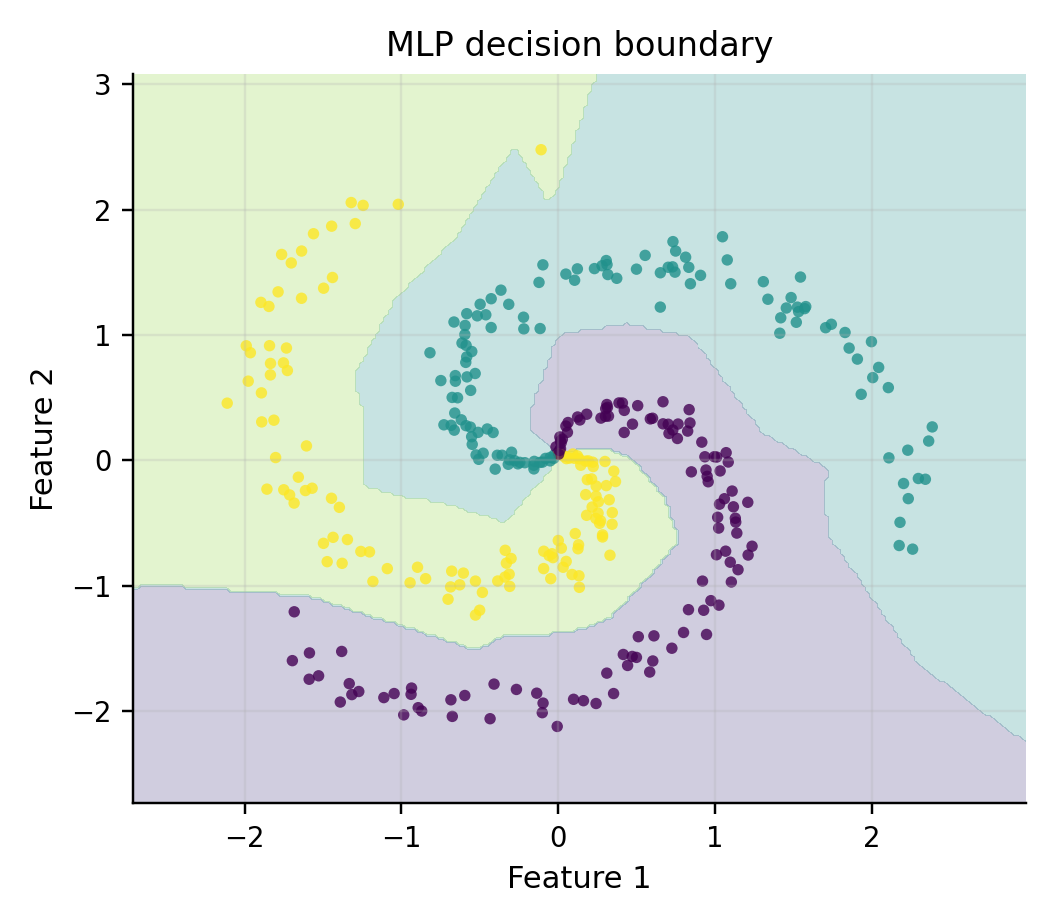
\includegraphics[width=0.58\linewidth]{figures/mlp_decision_boundary.png}
\caption{MLP 在螺旋数据集上的分类边界示例}
\end{figure}

\section{实验二：MNIST CNN}
\subsection{方法}
第二题使用 PyTorch 搭建两层卷积网络完成 MNIST 分类。为满足“分析多种情况并保留分析结果”的要求，实验分为两组：第一组比较 Adam、SGD、RMSprop 与多档学习率；第二组在固定优化策略下比较卷积核大小、通道宽度、BatchNorm、Dropout 和池化。

\subsection{结果}
优化器/学习率搜索中，最佳组合为 \texttt{rmsprop}，学习率 \texttt{0.0001}，测试准确率 98.96\%。架构消融中，最佳配置为 \texttt{kernel5\_c32-64\_bn\_do25\_pool}，测试准确率 99.15\%。

\begin{table}[H]
\centering
\caption{CNN 优化器与学习率搜索 Top 配置}
\begin{tabular}{lllll}
\toprule
优化器 & 学习率 & 训练准确率 & 测试准确率 & 测试损失 \\
\midrule
rmsprop & 0.0001 & 98.42\% & 98.96\% & 0.0332 \\
adam & 0.001 & 98.42\% & 98.94\% & 0.0305 \\
adam & 0.0005 & 98.34\% & 98.88\% & 0.0329 \\
rmsprop & 0.0005 & 97.51\% & 98.88\% & 0.0353 \\
rmsprop & 0.001 & 97.31\% & 98.74\% & 0.0381 \\
sgd & 0.01 & 98.19\% & 98.64\% & 0.0408 \\
\bottomrule
\end{tabular}

\end{table}

\begin{table}[H]
\centering
\caption{CNN 架构消融 Top 配置}
\begin{tabular}{lllll}
\toprule
配置 & 消融因素 & 参数量 & 测试准确率 & 测试损失 \\
\midrule
kernel5\_c32-64\_bn\_do25\_pool & kernel\_size & 455114 & 99.15\% & 0.0253 \\
wide\_k3\_c64-128\_bn\_do25\_pool & channels & 879114 & 99.07\% & 0.0289 \\
baseline\_k3\_c32-64\_bn\_do25\_pool & baseline & 421834 & 98.96\% & 0.0298 \\
no\_batch\_norm\_k3\_c32-64\_do25\_pool & batch\_norm & 421642 & 98.95\% & 0.0320 \\
dropout50\_k3\_c32-64\_bn\_pool & dropout & 421834 & 98.95\% & 0.0323 \\
dropout0\_k3\_c32-64\_bn\_pool & dropout & 421834 & 98.86\% & 0.0377 \\
narrow\_k3\_c16-32\_bn\_do25\_pool & channels & 207018 & 98.72\% & 0.0370 \\
\bottomrule
\end{tabular}

\end{table}

\begin{figure}[H]
\centering
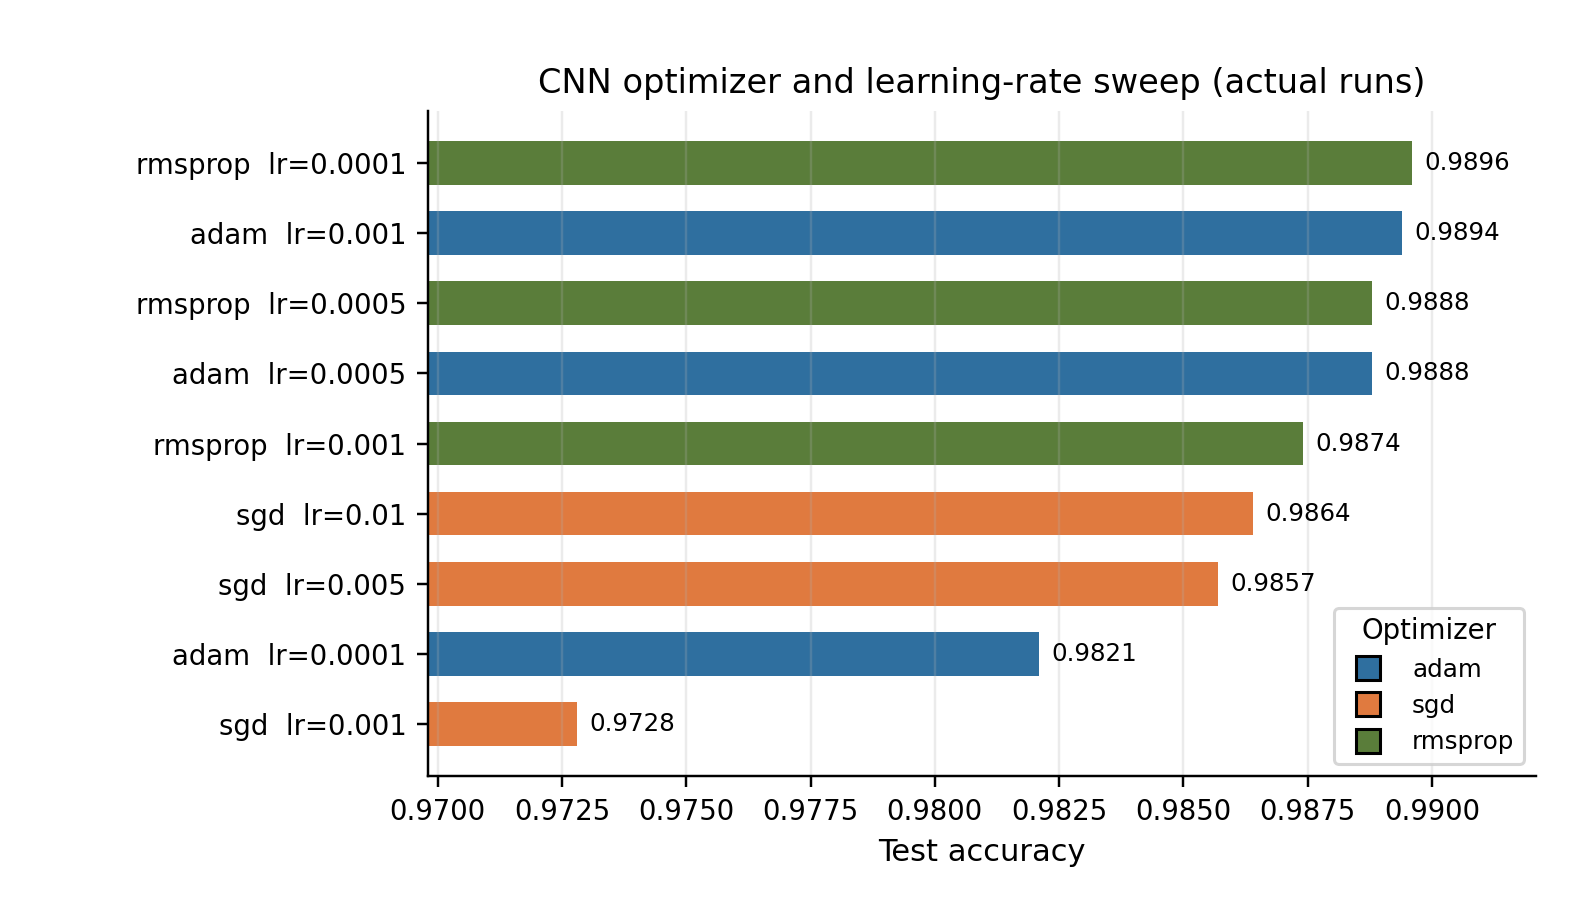
\includegraphics[width=0.72\linewidth]{figures/cnn_optimizer_lr_heatmap.png}
\caption{CNN 优化器与学习率真实运行配置排序图}
\end{figure}

\begin{figure}[H]
\centering
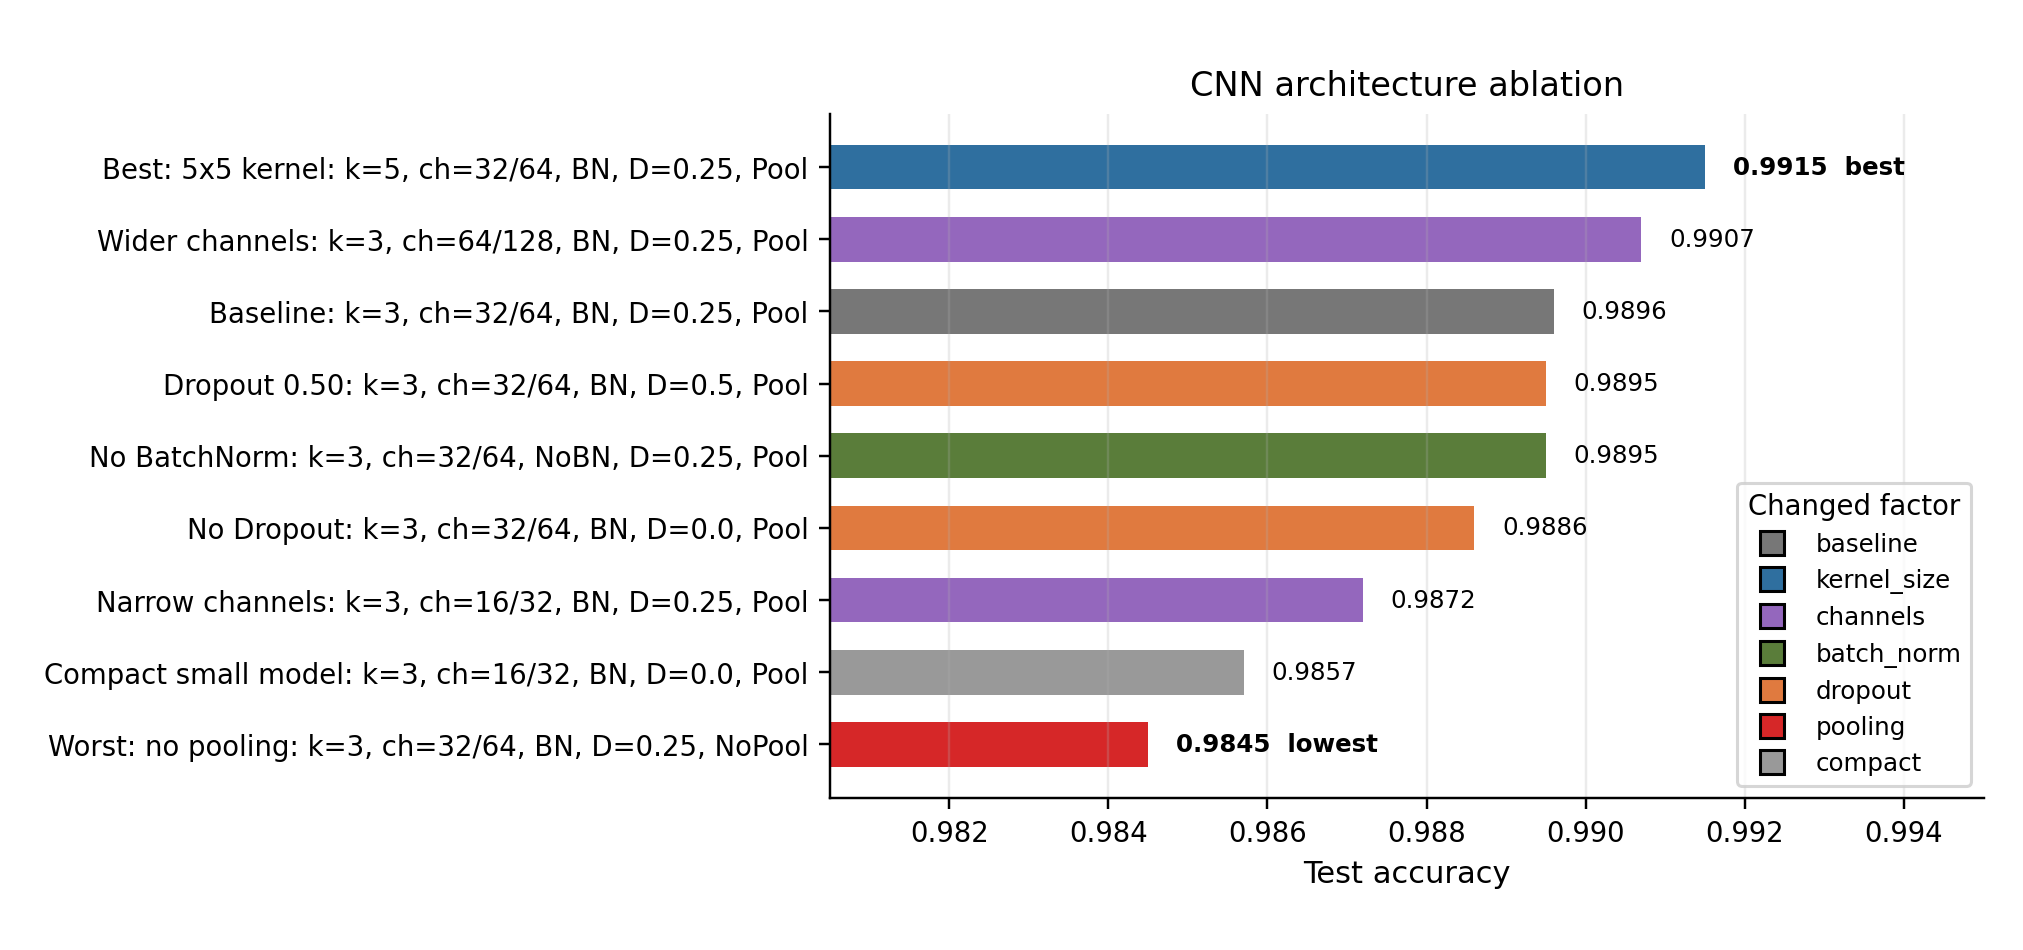
\includegraphics[width=0.88\linewidth]{figures/cnn_arch_ablation.png}
\caption{CNN 架构消融测试准确率，左侧直接标明配置变化}
\end{figure}

\section{实验三：ResNet-MNIST}
\subsection{方法}
第三题实现面向 MNIST 的 ResNet。基础提交保持 ResNet-50；扩展实验比较 ResNet-18、ResNet-34、ResNet-50，进一步加入无残差 Plain-18、ImageNet 风格 stem、不同优化器和学习率。这样既能覆盖任务书建议的 50 层残差网络，也能说明深度、残差连接和输入分辨率适配对结果的影响。

\subsection{结果}
ResNet sweep 中最佳配置为 \texttt{resnet34\_mnist\_adam\_1e-3}，测试准确率 99.31\%，参数量为 \texttt{21280970}。

\begin{table}[H]
\centering
\caption{ResNet 深度与结构消融结果}
\begin{tabular}{llllll}
\toprule
编号与配置 & 因素 & 参数量 & 优化器 & 学习率 & 测试准确率 \\
\midrule
R1: ResNet-34, MNIST, adam 0.001 & depth & 21280970 & adam & 0.001 & 99.31\% \\
R2: ResNet-18, MNIST, adam 0.001 & depth & 11172810 & adam & 0.001 & 99.17\% \\
R3: ResNet-18, MNIST, sgd 0.01 & optimizer & 11172810 & sgd & 0.01 & 99.16\% \\
R4: ResNet-18, MNIST, rmsprop 0.0001 & optimizer & 11172810 & rmsprop & 0.0001 & 98.94\% \\
R5: ResNet-18, ImageNet, adam 0.001 & stem & 11175370 & adam & 0.001 & 98.85\% \\
R6: ResNet-18, MNIST, adam 0.0005 & learning\_rate & 11172810 & adam & 0.0005 & 98.76\% \\
R7: ResNet-50, MNIST, adam 0.001 & depth & 23519690 & adam & 0.001 & 98.58\% \\
R8: Plain-18, MNIST, adam 0.001 & residual & 11172810 & adam & 0.001 & 97.81\% \\
\bottomrule
\end{tabular}

\end{table}

\begin{figure}[H]
\centering
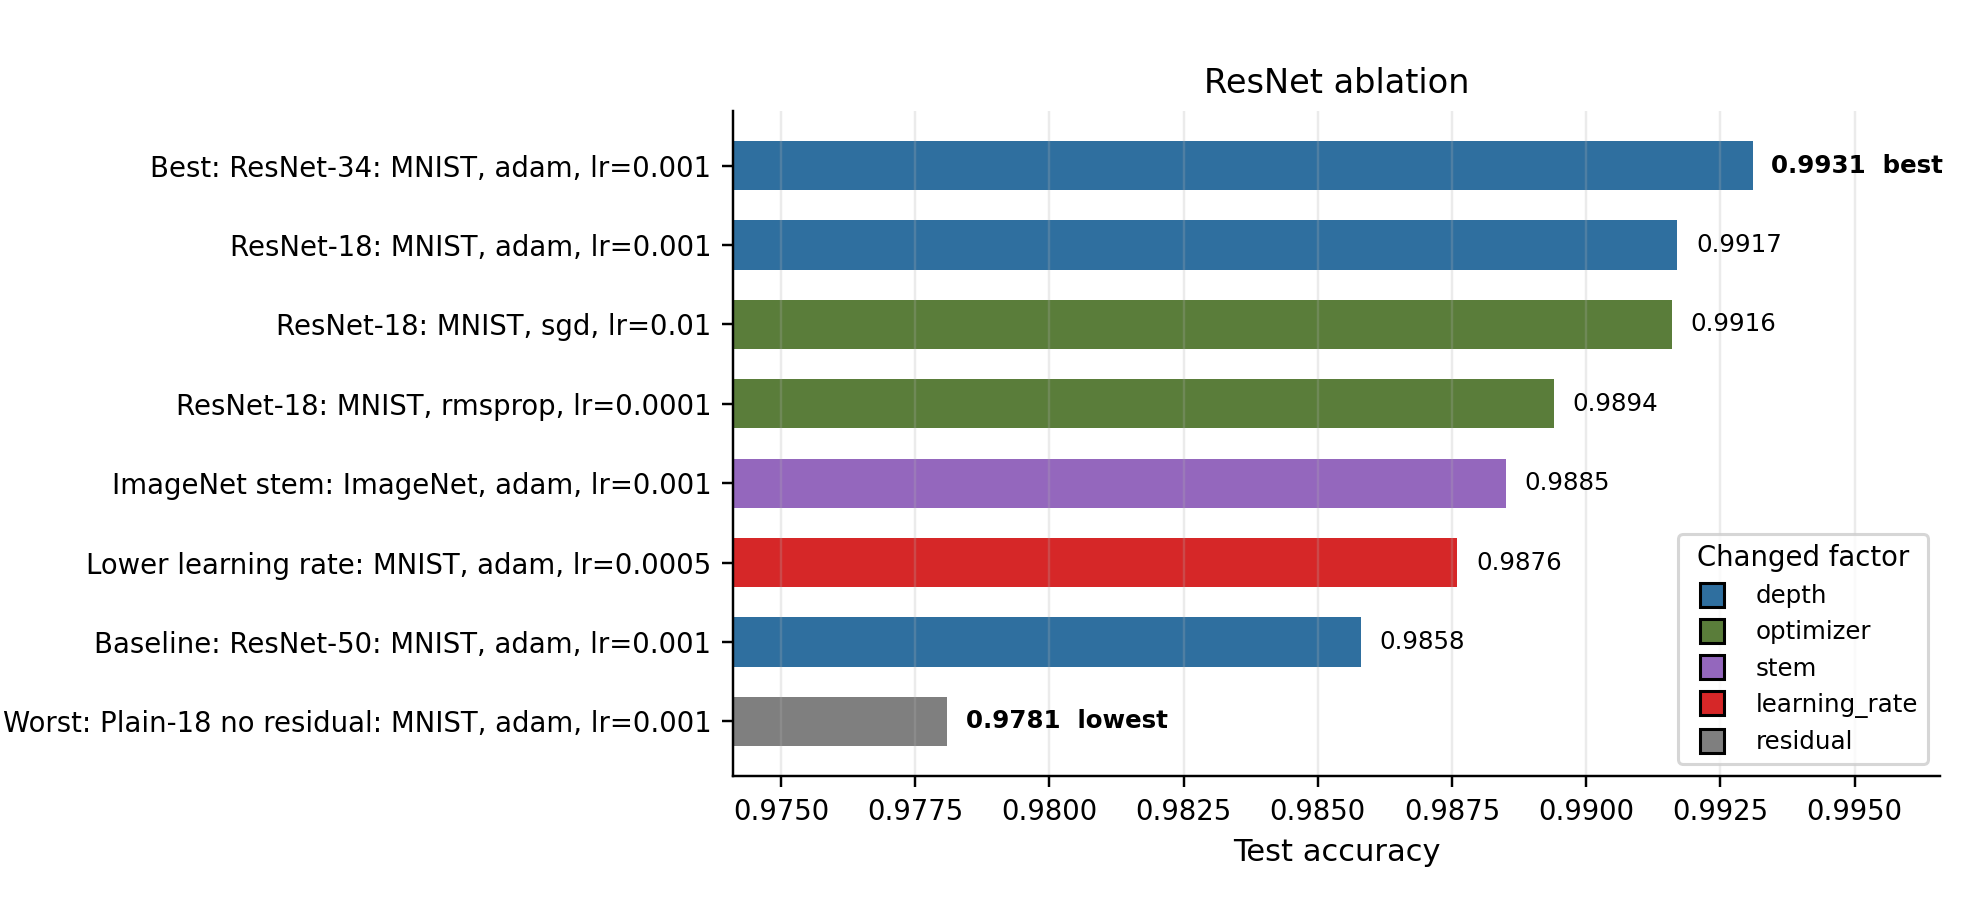
\includegraphics[width=0.88\linewidth]{figures/resnet_ablation.png}
\caption{ResNet 不同配置测试准确率，左侧直接标明模型变化}
\end{figure}

\begin{figure}[H]
\centering
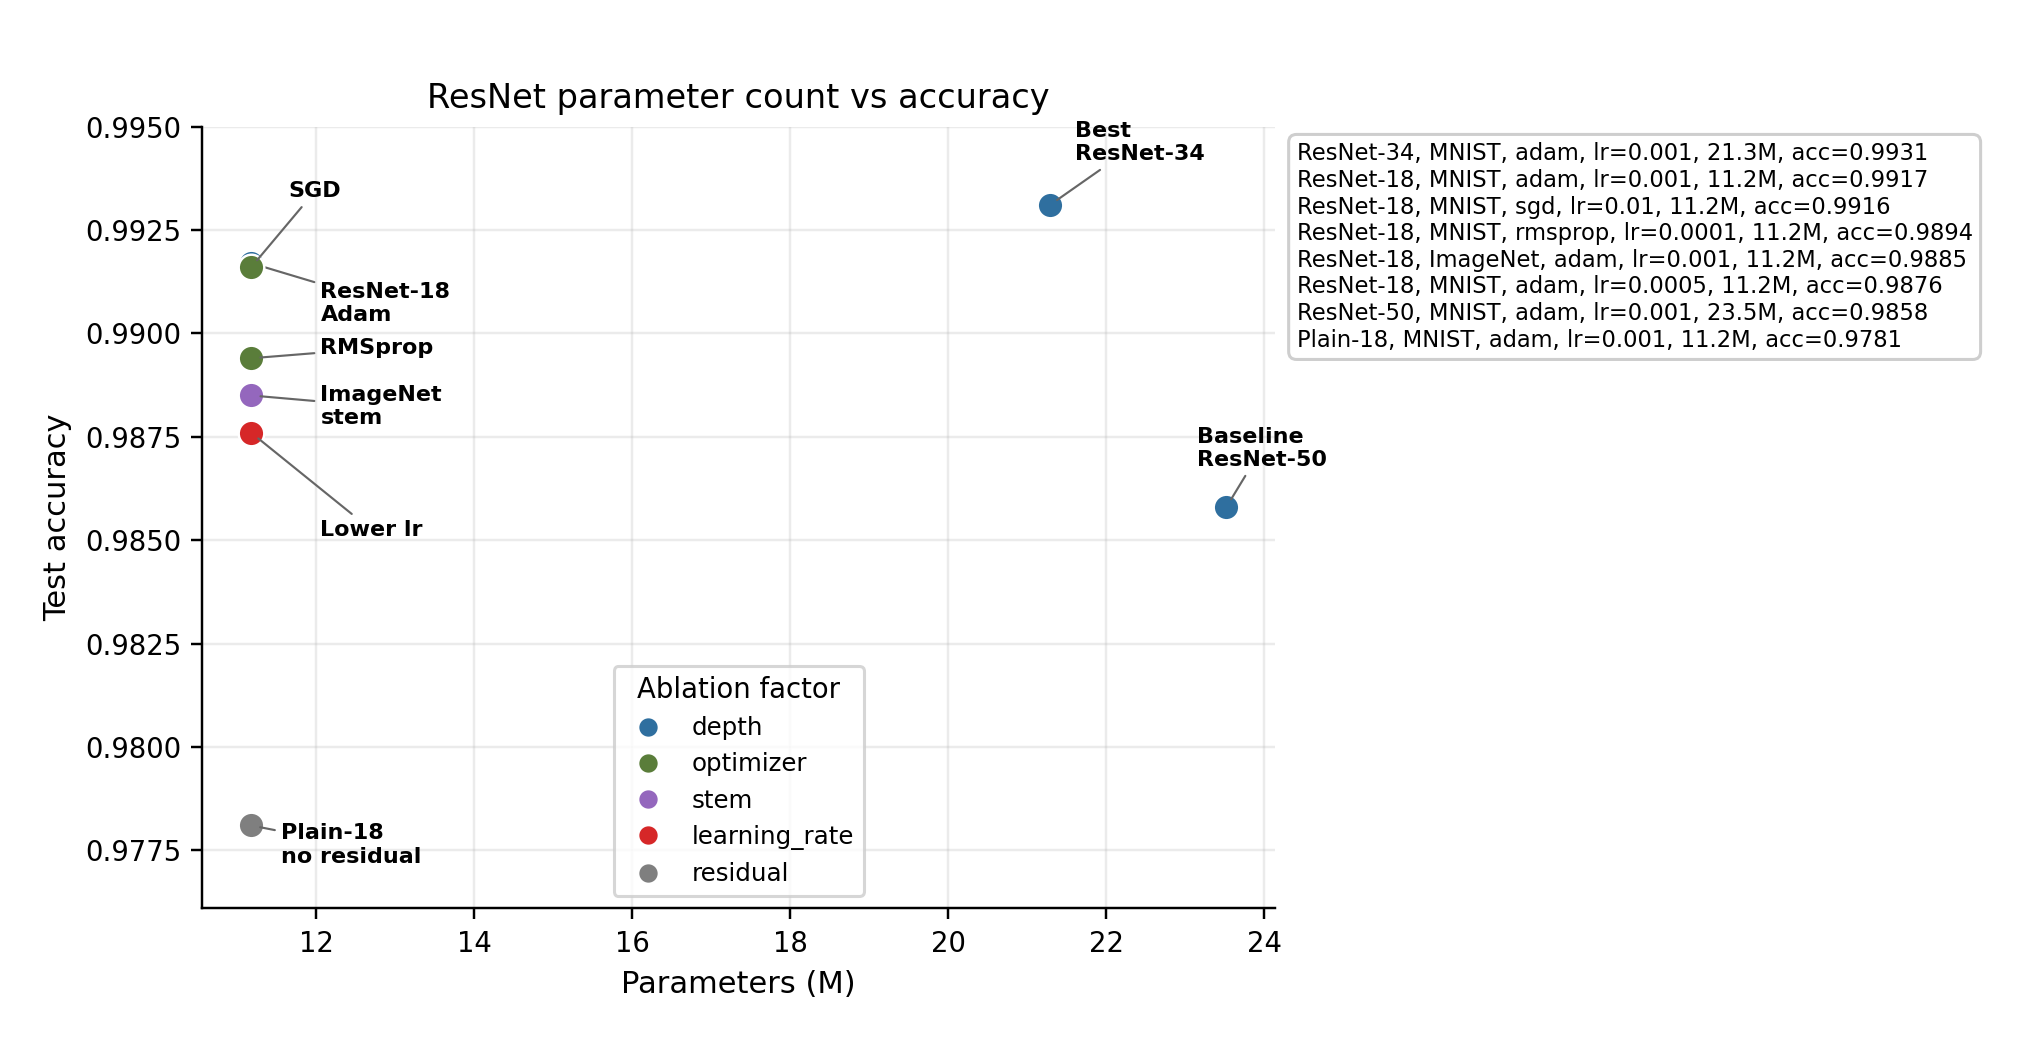
\includegraphics[width=0.80\linewidth]{figures/resnet_params_accuracy.png}
\caption{ResNet 参数量与测试准确率关系，点旁边直接标明模型含义}
\end{figure}

\section{综合分析与汇报思路}
汇报时建议先说明三部分递进关系：NumPy MLP 体现前向传播、损失函数和反向传播的底层实现；CNN 体现局部感受野和参数共享在图像识别上的效果；ResNet 体现残差连接对深层网络训练稳定性的作用。随后按“基础实现是否满足任务书要求、扩展对比实验如何设计、结果说明什么”展开。

从结果看，MNIST 上浅层 CNN 已经能够达到较高准确率，ResNet 的主要价值不只是单点准确率，而是通过深度、残差连接和 stem 对比展示深层网络设计原则。MLP 实验则显示，在非线性二维数据上，激活函数和优化器会显著影响收敛速度与分类边界质量。

\section{复现方式}
\begin{verbatim}
.conda-env/bin/python 01_numpy_mlp/run_experiment.py --epochs 1500
.conda-env/bin/python 01_numpy_mlp/sweep_mlp.py --epochs 1000
.conda-env/bin/python 02_mnist_cnn/train_cnn.py --epochs 3 --batch-size 256
.conda-env/bin/python 02_mnist_cnn/sweep_cnn.py --epochs 3 --batch-size 256 --num-workers 4
.conda-env/bin/python 02_mnist_cnn/sweep_arch_cnn.py --epochs 3 --batch-size 256 --num-workers 4
.conda-env/bin/python 03_resnet_mnist/train_resnet.py --epochs 3 --batch-size 256
.conda-env/bin/python 03_resnet_mnist/sweep_resnet.py --epochs 3 --batch-size 256 --num-workers 4
.conda-env/bin/python latex_report/build_report_assets.py
\end{verbatim}

\section{结论}
三个实验均完成了任务书目标，并进一步保留了多种实验条件下的结构化结果。报告材料能够支持课堂汇报和后续本地 LaTeX 编译；代码输出中的 JSON/CSV 文件可作为实验可复现证据。

\end{document}
